
\begin{figure}[ht!]
	\centering
	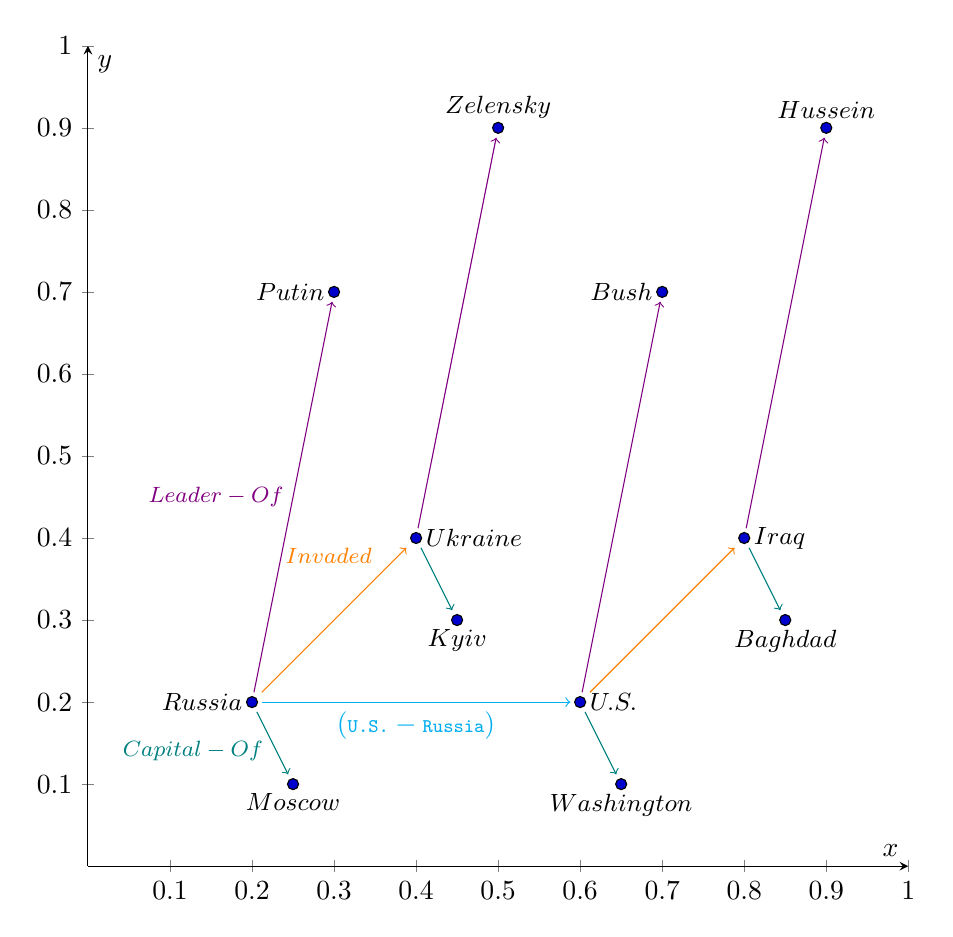
\begin{tikzpicture}
		\begin{axis}[axis lines=center,
			%view={28}{22},
			xmin=0, xmax=1, ymin=0, ymax=1,
			%xtick={0,1},ytick={0,1.0},
			xlabel=$x$,ylabel=$y$,width=12cm,height=12cm]
			\addplot+[only marks,point meta=explicit symbolic, nodes near coords,black] coordinates 
			{
				% Putin
				(0.3,0.7)[]
				% Russia
				(0.2,0.2)[]
				% Moscow
				(0.25,0.1)[]
				% Ukraine
				(0.4,0.4)[]
				% Kyiv
				(0.45,0.3)[]
				% Zelensky
				(0.5,0.9)[{\small$\entvecpgf{Zelensky}$}]
				% Bush
				(0.7,0.7)[]
				% US
				(0.6,0.2)[]
				% Washington
				(0.65,0.1)[]
				% Iraq
				(0.8,0.4)[]
				% Baghdad
				(0.85,0.3)[]
				% Hussein
				(0.9,0.9)[{\small$\entvecpgf{Hussein}$}]
			};
			%\node[anchor=west] (source) at (axis cs:0.0,0.0){};
			% Russia + Label
			\node (russia) at (axis cs:0.2,0.2){};
			\node[anchor=east] (russial) at (axis cs:0.2,0.2){{\small$\entvecpgf{Russia}$}};
			% Moscow + Label
			\node (moscow) at (axis cs:0.25,0.1){};
			\node[anchor=north] (moscowl) at (axis cs:0.25,0.1){{\small$\entvecpgf{Moscow}$}};
			% Ukraine + Label
			\node (ukraine) at (axis cs:0.4,0.4){};
			\node[anchor=west] (ukrainel) at (axis cs:0.4,0.4){{\small$\entvecpgf{Ukraine}$}};
			% Kyiv + Label
			\node (kyiv) at (axis cs:0.45,0.3){};
			\node[anchor=north] (kyivl) at (axis cs:0.45,0.3){{\small$\entvecpgf{Kyiv}$}};
			% Putin + Label
			\node (putin) at (axis cs:0.3,0.7){};
			\node[anchor=east] (putinl) at (axis cs:0.3,0.7){{\small$\entvecpgf{Putin}$}};
			% Zelensky
			\node (zelen) at (axis cs:0.5,0.9){};
			% US + Label
			\node (us) at (axis cs:0.6,0.2){};
			\node[anchor=west] (usl) at (axis cs:0.6,0.2){{\small$\entvecpgf{U.S.}$}};
			% Washington + Label
			\node (wash) at (axis cs:0.65,0.1){};
			\node[anchor=north] (washl) at (axis cs:0.65,0.1){{\small$\entvecpgf{Washington}$}};
			% Iraq + Label
			\node (iraq) at (axis cs:0.8,0.4){};
			\node[anchor=west] (iraql) at (axis cs:0.8,0.4){{\small$\entvecpgf{Iraq}$}};
			% Baghdad + Label
			\node (baghdad) at (axis cs:0.85,0.3){};
			\node[anchor=north] (baghdadl) at (axis cs:0.85,0.3){{\small$\entvecpgf{Baghdad}$}};
			% Bush + Label
			\node (bush) at (axis cs:0.7,0.7){};
			\node[anchor=east] (bushl) at (axis cs:0.7,0.7){{\small$\entvecpgf{Bush}$}};
			% Hussein
			\node (hussein) at (axis cs:0.9,0.9){};
			%%% Arrow labels
			% Invaded
			\node[anchor=north west,color=orange] (invaded) at (axis cs:0.229,0.4){{\footnotesize$\relvecpgf{Invaded}$}};
			% US-Russia
			\node[anchor=north,color=cyan] (usmrus) at (axis cs:0.4,0.2){$\left(\vv{\scriptsize{\texttt{U.S.}}}-\vv{\scriptsize{\texttt{Russia}}}\right)$};
			% Leader
			\node[anchor=east,color=violet] (leader) at (axis cs:0.25,0.45) {{\footnotesize$\relvecpgf{Leader-Of}$}};
			% Capital
			\node[anchor=east, color=teal] (capital) at (axis cs:0.225,0.14) {{\footnotesize$\relvecpgf{Capital-Of}$}};
			\draw[->,color=orange](russia)--(ukraine);
			\draw[->,color=violet](russia)--(putin);
			\draw[->,color=teal](russia)--(moscow);
			\draw[->,color=cyan](russia)--(us);
			\draw[->,color=violet](ukraine)--(zelen);
			\draw[->,color=teal](ukraine)--(kyiv);
			%\draw[->,color=orange](putin)--(zelen);
			\draw[->,color=orange](us)--(iraq);
			\draw[->,color=violet](us)--(bush);
			\draw[->,color=teal](us)--(wash);
			\draw[->,color=violet](iraq)--(hussein);
			\draw[->,color=teal](iraq)--(baghdad);
			%\draw[->,color=orange](bush)--(hussein);
		\end{axis}
	\end{tikzpicture}
	\caption{A visualization of the ``analogical math'' which can be performed within word embedding spaces, due to their ability to capture multiple \textit{types} of word-word relationships in the form of distances ranging over multiple dimensions: entity vectors are typeset in fixed-width font ($\entvec{Entity}$), while relational vectors are typeset in serif font ($\relvec{Relation}$). The vector from $\entvec{Russia}$ to $\entvec{U.S.}$, a relational vector, is typeset in fixed-width font only to illustrate its mathematical form (i.e., that it is computed via the subtraction two entity vectors).}
	\label{fig:nyt-vectors}
\end{figure}